
\documentclass[letterpaper, reqno,11pt]{article}
\usepackage[margin=1.0in]{geometry}
\usepackage{color,latexsym,amsmath,amssymb}
\usepackage{fancyhdr}
\usepackage{amsthm}
\usepackage[linesnumbered,lined,boxed,commentsnumbered,noend,noline]{algorithm2e}
\usepackage{dsfont}
\usepackage{graphicx}
\usepackage{hyperref}
\usepackage{bbm}
\usepackage[inline]{enumitem}
\usepackage[numbers]{natbib}
\usepackage{framed}
\usepackage{titling}
\usepackage{subcaption}
\usepackage[dvipsnames]{xcolor}
\usepackage{tikz}
\usetikzlibrary{hobby}
\usetikzlibrary{shapes.multipart}
\usepackage{pgfplots}
\pgfplotsset{compat=1.7}
\usetikzlibrary{arrows.meta}
\usetikzlibrary{decorations.markings}
\usetikzlibrary{shapes}
\usetikzlibrary{arrows}
\usepgfplotslibrary{fillbetween}
\usetikzlibrary{patterns}

\tikzset{invclip/.style={clip,insert path={{[reset cm]
  (-16383.99999pt,-16383.99999pt) rectangle (16383.99999pt,16383.99999pt)}}}}

\allowdisplaybreaks

\newcommand{\RR}{\mathbb{R}}
\newcommand{\CC}{\mathbb{C}}
\newcommand{\ZZ}{\mathbb{Z}}
\newcommand{\QQ}{\mathbb{Q}}
\newcommand{\NN}{\mathbb{N}}
\newcommand{\FF}{\mathbb{F}}
\newcommand{\PP}{\mathop{{}\mathbb{P}}}
\newcommand{\EE}{\mathop{{}\mathbb{E}}}
\newcommand{\LL}{\mathbb{L}}
\newcommand{\TT}{\mathbb{T}}
\newcommand{\GI}{\textrm{GI}}
\newcommand{\coGI}{\overline{\textrm{GI}}}
\DeclareMathOperator{\conv}{conv}
\DeclareMathOperator{\charcone}{char.cone}
\DeclareMathOperator{\STAB}{STAB}
\DeclareMathOperator{\Down}{Down}
\DeclareMathOperator{\lca}{lca}
\DeclareMathOperator{\ex}{ex}
\DeclareMathOperator{\Span}{span}
\DeclareMathOperator{\T}{\mathsf{T}}
\DeclareMathOperator{\F}{\mathsf{F}}
\DeclareMathOperator{\shP}{\# P}
\DeclareMathOperator{\shSAT}{\# SAT}
\DeclareMathOperator{\shDNF}{\# DNF}
\DeclareMathOperator{\DNF}{\textsf{DNF}}
\DeclareMathOperator{\Poly}{\textsf{P}}
\DeclareMathOperator{\CNF}{\textsf{CNF}}
\DeclareMathOperator{\SAT}{\textsf{SAT}}
\DeclareMathOperator{\BPP}{\textsf{BPP}}
\DeclareMathOperator{\poly}{poly}
\DeclareMathOperator{\RP}{\textsf{RP}}
\DeclareMathOperator{\EXP}{\textsf{EXP}}
\DeclareMathOperator{\DTIME}{\textsf{DTIME}}
\DeclareMathOperator{\NP}{\textsf{NP}}
\DeclareMathOperator{\MCprime}{MC'}
\DeclareMathOperator{\Var}{Var}
\DeclareMathOperator{\IP}{\textsf{IP}}
\DeclareMathOperator{\PSPACE}{\textsf{PSPACE}}
\DeclareMathOperator{\lollipop}{lollipop}
\DeclareMathOperator{\ustconn}{\textsf{UST-Conn}}
\DeclareMathOperator{\RL}{\textsf{RL}}
\DeclareMathOperator{\dist}{dist}
\DeclareMathOperator{\Ex}{Ex}
\DeclareMathOperator{\error}{error}
\DeclareMathOperator{\AND}{\mathsf{AND}}
\DeclareMathOperator{\ANDbar}{\mathsf{\overline{AND}}}
\DeclareMathOperator{\val}{val}
\DeclareMathOperator{\sign}{sign}
\DeclareMathOperator{\NS}{NS}
\DeclareMathOperator{\Maj}{Maj}
\DeclareMathOperator{\Inf}{Inf}
\DeclareMathOperator{\WL}{WL}
\DeclareMathOperator{\SL}{\textsc{StrongLearn}}
\newcommand\mycommfont[1]{\ttfamily\textcolor{blue}{#1}}
\SetCommentSty{mycommfont}
\SetKwFor{RepTimes}{repeat}{times}{end}
\begin{document}
\pagenumbering{arabic}
\title{Lectures on Learning Theory}
\author{Yuchong Pan}
\date{\today}
\newtheorem{theorem}{Theorem}
\newtheorem{lemma}[theorem]{Lemma}
\newtheorem{proposition}[theorem]{Proposition}
\newtheorem{corollary}[theorem]{Corollary}
\newtheorem{fact}[theorem]{Fact}
\newtheorem{problem}[theorem]{Problem}
\newtheorem{observation}[theorem]{Observation}
\newtheorem{claim}{Claim}
\newtheorem{exercise}{Exercise}
\theoremstyle{definition}
\newtheorem{definition}[theorem]{Definition}
%\maketitle
%

\begin{framed}
\noindent{\bf 6.842 Randomness and Computation} \hfill \thedate
\begin{center}
\Large{\thetitle}
\end{center}
\noindent{\em Lecturer: Ronitt Rubinfield} \hfill {\em Scribe: \theauthor}
\end{framed}

\section{PAC Learning}

The model of \emph{learning from random, uniform examples} is as follows: Given the \emph{example oracle} $\Ex(f)$ of a function $f$, pick $m$ i.i.d.\ random variables $x_1, \ldots, x_m$ uniformly (or from some distribution $\mathcal D$, which might not be known to the learner in general), and call $\Ex(f)$ to obtain $m$ random labeled examples $(x_1, f(x_1)), \ldots, (x_m, f(x_m))$; after seeing these examples, the learner outputs a hypothesis $h$ of the function $f$.

Should we require $h = f$? This is probably too much to ask. However, we can at least require $\dist(h, f) := \PP_{x \sim \mathcal D}(h(x) \neq f(x)) \leq \varepsilon$, where $\dist(h, f)$ is also called $\error_{\mathcal D}(h)$ with respect to $f$.

\begin{definition}
  A \emph{uniform distribution learning algorithm for a concept class $\mathcal C$} is an algorithm $\mathcal A$ that, given $\varepsilon > 0$, $\delta > 0$ and access to $\Ex(f)$ for $f \in \mathcal C$, outputs a function $h$ such that with probability at least $1 - \delta$, $\error(h)$ with respect to $f$ is at most $\varepsilon$. This is called \emph{probably approximately correct (PAC) learning}.
\end{definition}

We are interested in the following parameters:
\begin{itemize}[itemsep=0pt]
  \item $m$, the \emph{sample complexity};
  \item $\varepsilon$, the \emph{accuracy} parameter;
  \item $\delta$, the \emph{confidence} parameter;
  \item the running time, which we hope to be $\poly(\log(\text{domain size}), 1/\varepsilon, 1/\delta)$;
  \item the \emph{description} of $h$, which at least should be compact (i.e., $O(\log |\mathcal C|)$) and efficient to evaluate; it require $h \in \mathcal C$, then this is called \emph{proper learning}.
\end{itemize}
Note that the uniform case is a special case of the PAC model. The more general PAC model is given $\Ex_{\mathcal D}(f)$ and bounds $\error_{\mathcal D}(h)$ with respect to $f$.

\section{Learning Conjunctions}

Let $\mathcal C$ be the class of conjunctions (i.e., $1$-term DNF) over $\{ 0, 1 \}^n$. We cannot hope for $0$-error from a sub-exponential number of random samples; to see this, note that it is hard to distinguish $f(x) = x_1 \cdots x_n$ and $f(x) = \F$. Algorithm \ref{alg:conjunction} gives a polynomial time sampling algorithm for conjunction learning, where ``\textcolor{red}{\bf ?}'' indicates a parameter to be determined.

\begin{algorithm}
  draw $\poly(1/\varepsilon)$ samples \\
  estimate $\PP[f(x) = 1]$ to additive error at most $\pm \varepsilon/4$ and confidence at least $1 - \delta/2$ \\
  \If{estimate is less than $\varepsilon/2$}{
    \Return{$h(x) = 0$}
  }
  \CommentSty{(estimate is at least $\varepsilon/2$; see a new positive example every $O(1/\varepsilon)$ samples)} \\
  collect \textcolor{red}{\bf ?} more positive examples \\
  $V \leftarrow \text{set of indices of variables that are set in the same way in each positive example}$ \\
  \Return{$h(x) = \bigwedge_{i \in V} x_i^{b_i}$, where each $b_i$ indicates if $x_i$ is complemented or not}
  \caption{A polynomial time sampling algorithm for conjunction learning.}
  \label{alg:conjunction}
\end{algorithm}

For $x_i$ in the conjunction, it must be set in the same way in each positive example, so $i \in V$. For $x_i$ not in the conjunction,
$$ \PP[i \in V] = \PP\left[\text{$x_i$ is set is the same way in each of the $k$ positive examples}\right] = \frac{1}{2^{k - 1}}. $$
By the union bound,
$$ \PP\left[\text{any $x_i$ not in the conjunction survives}\right] \leq \frac{n}{2^{k - 1}} \leq \delta, $$
if we pick $k = \log (n/\delta)$. Therefore, if we need $\Omega(\log(n/\delta))$ positive examples, or $\Omega((1/\varepsilon) \log(n/\delta))$ total examples to rule out every $x_i$ not in the conjunction.

\section{Occam's Razor}

In a high level, \emph{Occam's Razor} claims the following:
\begin{itemize}[itemsep=0pt]
  \item If we ignore the running time, then learning is easy (with a polynomial number of samples).
  \item The shortest explanation is the best.
\end{itemize}
To see the first claim, we consider the brute-force algorithm in Algorithm \ref{alg:occam}.

\begin{algorithm}
  draw $M = (1/\varepsilon) (\ln |\mathcal C| + \ln |1/\delta|)$ \\
  search over all $h \in \mathcal C$ until find one consistent with the samples \\
  \Return{$h$}
  \caption{A brute-force learning algorithm that demonstrates Occam's Razor.}
  \label{alg:occam}
\end{algorithm}

We say that a function $h$ is \emph{bad} if $\error(h)$ with respect to $f$ is at least $\varepsilon$. For a bad function $h$,
$$ \PP[\text{$h$ is consistent with the samples}] \leq (1 - \varepsilon)^M. $$
By the union bound,
$$ \PP[\text{any bad function $h$ is consistent with the samples}] \leq |\mathcal C| (1 - \varepsilon)^M = |\mathcal C| (1 - \varepsilon)^{\frac{1}{\varepsilon}\left(\ln |\mathcal C| + \ln \left|\frac{1}{\delta}\right|\right)} = \delta. $$
Hence, it is unlikely to output a bad hypothesis $h$. For example, for conjunction learning, this analysis requires $O((1/\varepsilon)(n + 1/\delta))$ samples, where Algorithm \ref{alg:conjunction} has a better sample complexity. On the other hand, if we have a \emph{good} hypothesis $h$,
\begin{enumerate}[label=(\roman*), itemsep=0pt]
  \item we can \emph{predict} values of $f$ on new random inputs according to distribution $\mathcal D$, since
  $$ \PP_{x \sim \mathcal D}[f(x) = h(x)] \geq 1 - \delta; $$
  \item we can \emph{compress} the description of samples $(x_1, f(x_1)), (x_2, f(x_2)), \ldots, (x_m, f(x_m))$ from the na\"ive description which takes $m(\log |D| + \log |R|)$ bits, where $D$ and $R$ are the domain and the range of $f$, respectively, to the form ``$x_1, \ldots, x_m$ plus the description of $h$'' which requires $m\log |D| + \log |\mathcal C|$ bits only.
\end{enumerate}

\section{Learning via Fourier Representations}

In this section, we study learning algorithms that are based on estimating the Fourier representation of a function $f$.

\subsection{Approximating One Fourier Coefficient}

\begin{lemma}
  For any $S \subset [n]$, one can approximate $\hat{f}(S)$ to within additive error $\gamma$ (i.e., $|\text{output} - \hat{f}(S)| \leq \gamma$) with probability at least $1 - \delta$ in $O(1/\gamma^2 \log 1/\delta)$ samples.
\end{lemma}

\begin{proof}
  Recall that $\hat{f}(S) = 2\PP_{x \in \{ 0, 1 \}^n}[f(x) \neq \chi_S(x)] - 1$. Hence, we can approximate $\hat{f}(S)$ by estimating $\PP_{x \in \{ 0, 1 \}^n}[f(x) \neq \chi_S(x)]$ and applying the Chernoff bound.
\end{proof}

\subsection{Fourier Concentration and the Low Degree Algorithm}

\begin{definition}
  For all $\varepsilon \in (0, 1)$ and $n \in \NN$, we say that a function $f : \{ \pm 1 \}^n \to \RR$ has \emph{$\alpha(\varepsilon, n)$-Fourier concentration (f.c.)} if
  $$ \sum_{\substack{S \subset [n] \\ |S| > \alpha(\varepsilon, n)}} \hat{f}(S)^2 \leq \varepsilon. $$
\end{definition}

For a Boolean function $f : \{ \pm 1 \}^n \to \{ \pm 1 \}$, Parseval's identity gives $\sum_{S \subset [n]} \hat{f}(S)^2 = 1$, so having $\alpha(\varepsilon, n)$-Fourier concentration implies that
$$ \sum_{\substack{S \subset [n] \\ |S| \leq \alpha(\varepsilon, n)}} \geq 1 - \varepsilon. $$

The \emph{low degree algorithm}, given in Algorithm \ref{alg:low-degree}, approximates a Boolean function with $d$-Fourier concentration, where $d = \alpha(\varepsilon, n)$.

\begin{algorithm}
  take $m = O((n^d/\tau) \log (n^d/\delta))$ samples \\
  \ForEach{$S \subset [n]$ such that $|S| \leq d$}{
    $C_S \leftarrow \text{estimate of $\hat{f}(S)$}$
  }
  let $h : \{ \pm 1 \}^n \to \RR$ be defined by $h(x) = \sum_{S \subset [n] : |S| \leq d} C_S \chi_S(x)$ \\
  \Return{$\sign \circ h$ as hypothesis}
  \caption{The low degree algorithm given degree $d$, accuracy $\tau$ and confidence $\delta$.}
  \label{alg:low-degree}
\end{algorithm}

\begin{proposition} \label{prop:expectation}
  If $f$ has $d$-Fourier concentration with $d = \alpha(\varepsilon, n)$, then $\EE_{x \in \{ 0, 1 \}^n} [(f(x) - h(x))^2] \leq \varepsilon + \tau$ with probability at least $1 - \delta$.
\end{proposition}

\begin{proof}
  First, we claim that each low degree Fourier Coefficient is well approximated, i.e., with probability at least $1 - \delta$, we have $|C_S - \hat{f}(S)| \leq \gamma$ for all $S \subset [n]$ with $|S| \leq d$, where $\gamma = \sqrt{\tau/n^d}$. This can be proved using the Chernoff bound and the union bound.

  Second, we show that if all low degree Fourier coefficients are well approximated, then $h$ has a low $\ell_2$-error. Suppose $|C_S - \hat{f}(S)| \leq \gamma$ for all $S \subset [n]$ such that $|S| \leq d$. Let $g : \{ \pm 1 \}^n \to \RR$ be defined by
  $$ g(x) = f(x) - h(x). $$
  By the linearity of the Fourier transform, for all $S \subset [n]$,
  $$ \hat{g}(S) = \hat{f}(S) - \hat{h}(S). $$
  For all $S \subset [n]$ with $|S| > d$, we have $\hat{h}(S) = 0$, so $\hat{g}(S) = \hat{f}(S)$. For all $S \subset [n]$ with $|S| \leq d$, we have $|\hat{g}(S)| \leq \gamma$, so $\hat{g}(S)^2 \leq \gamma^2$. Therefore,
  \begin{align*}
    \EE_{x \in \{ \pm 1 \}^n}\left[(f(x) - h(x))^2\right] &= \EE\left[g(x)^2\right] = \sum_{S \subset [n]} \hat{g}(S)^2 && \text{(Parseval's identity)} \\
    &= \sum_{\substack{S \subset [n] \\ |S| \leq d}} \hat{g}(S)^2 + \sum_{\substack{S \subset [n] \\ |S| > d}} \hat{g}(S)^2 \\
    &\leq \sum_{\substack{S \subset [n] \\ |S| \leq d}} \gamma^2 + \sum_{\substack{S \subset [n] \\ |S| > d}} \hat{f}(S)^2 \\
    &\leq \binom{n}{d} \cdot \gamma^2 + \varepsilon && \text{(by Fourier concentration)} \\
    &\leq \tau + \varepsilon.
  \end{align*}
  This completes the proof.
\end{proof}

\begin{proposition} \label{prop:prob}
  Let $f : \{ \pm 1 \}^n \to \{ \pm 1 \}$. Let $h : \{ \pm 1 \}^n \to \RR$. Then
  $$ \PP_{x \in \{ \pm 1 \}^n} [f(x) \neq \sign(h(x))] \leq \EE_{x \in \{ \pm 1 \}^n}\left[(f(x) - h(x))^2\right] $$
\end{proposition}

\begin{proof}
  Recall that
  \begin{align}
    \EE_{x \in \{ \pm 1 \}^n}\left[(f(x) - h(x))^2\right] &= \frac{1}{2^n} \sum_{x \in \{ \pm 1 \}^n} (f(x) - h(x))^2, \label{eq:expecation} \\
    \PP_{x \in \{ \pm 1 \}^n} \left[f(x) \neq \sign(h(x))\right] &= \frac{1}{2^n} \sum_{x \in \{ \pm 1 \}^n} \mathds 1_{f(x) \neq \sign(h(x))}. \label{eq:prob}
  \end{align}
  We compare \eqref{eq:expecation} and \eqref{eq:prob} term by term. Let $x \in \{ \pm 1 \}^n$. If $f(x) = \sign(h(x))$, then $\mathds 1_{f(x) \neq \sign(h(x))} = 0 \leq (f(x) - h(x))^2$. If $f(x) \neq \sign(h(x))$, then $\mathds 1_{f(x) \neq \sign(h(x))} = 1 \leq (f(x) - h(x))^2$; see Figure \ref{fig:proof-prob} for an illustration.

  \begin{figure}[h]
    \centering
    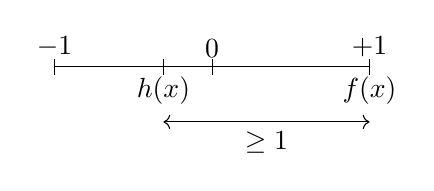
\begin{tikzpicture}
      \draw (-2, 0) -- (2, 0);
      \draw (-2, -.1) -- (-2, .1);
      \draw (0, -.1) -- (0, .1);
      \draw (2, -.1) -- (2, .1);
      \draw (-.618, -.1) -- (-.618, .1);
      \node[above] at (-2, 0) {$-1$};
      \node[above] at (0, 0) {$0$};
      \node[above] at (2, 0) {$+1$};
      \node[below] at (-.618, 0) {$h(x)$};
      \node[below] at (2, 0) {$f(x)$};
      \draw[<->] (-.618, -.7) -- (2, -.7) node[midway, below] {$\geq 1$};
    \end{tikzpicture}
    \caption{Illustrating the proof of Proposition \ref{prop:prob}.}
    \label{fig:proof-prob}
  \end{figure}
\end{proof}

\begin{theorem}
  If a concept class $\mathcal C$ has Fourier concentration $d = \alpha(\varepsilon, n)$, then there exists a uniform distribution learning algorithm for $\mathcal C$ with $q = O((n^d/\varepsilon) \log (n^d/\delta))$ samples; i.e., this algorithm gets $q$ samples and with probability at least $1 - \delta$ outputs a hypothesis $h'$ such that
  $$ \PP_{x \in \{ \pm 1 \}^n} \left[f(x) \neq h'(x)\right] \leq 2\varepsilon. $$
\end{theorem}

\begin{proof}
  Run the low degree algorithm with $\tau = \varepsilon$. By Proposition \ref{prop:expectation}, we get a hypothesis $h$ such that $\EE_{x \in \{ \pm 1 \}^n} [(f(x) - h(x))^2] \leq \varepsilon + \varepsilon = 2\varepsilon$. Let $h' = \sign \circ h$. By Proposition \ref{prop:prob}, $h'$ has error at most $2\varepsilon$ with respect to $f$. This completes the proof.
\end{proof}

Following are examples of functions that have $\alpha(\varepsilon, n)$-Fourier concentration.
\begin{enumerate}[label=(\roman*)]
  \item Any function $f : \{ \pm 1 \}^n \to \RR$ that depends on at most $k$ variables has
  $$ \sum_{\substack{S \subset [n] \\ |S| > k}} \hat{f}(S)^2 = 0. $$
  \item Let $T = \{ i_1, \ldots, i_k \} \subset [n]$ be such that $|T| = k$. Let $\AND : \{ \pm 1 \}^n \to \{ \pm 1 \}$ be defined by
  $$ \AND(x) = \left\{
    \begin{array}{ll}
      -1, & \text{if $x_i = -1$ for all $i \in T$}, \\
      1, & \text{otherwise}.
    \end{array}
  \right. $$
  We claim that $\AND$ has $\log(4/\varepsilon)$-Fourier concentration. Note $\widehat{\AND}(S) = 0$ for all $S \subset [n]$ with $|S| > |T|$. If $|T| \leq \log(4/\varepsilon)$, then we are done by definition. If $|T| > \log (4/\varepsilon)$, then
  $$ \widehat{\AND}(\emptyset)^2 = \left(1 - 2\PP\left[f(x) \neq \chi_\emptyset(x)\right]\right)^2 = \left(1 - 2 \cdot \frac{1}{2^{|T|}}\right)^2 > 1 - \varepsilon. $$
  Therefore, $\AND$ has $0$-Fourier concentration.
  \item Let $T = \{ i_1, \ldots, i_k \} \subset [n]$ be such that $|T| = k$. Let $\ANDbar : \{ \pm 1 \}^n \to \{ \pm 1 \}$ be defined by
  $$ \ANDbar(x) = \left\{
    \begin{array}{ll}
      1, & \text{if $x_i = -1$ for all $i \in T$}, \\
      -1, & \text{otherwise}.
    \end{array}
  \right. $$
  Let $f : \{ \pm 1 \}^n \to \{ 0, 1 \}$ be defined by
  \begin{align*}
    f(x) &= \left\{
      \begin{array}{ll}
        1, & \text{if $x_i = -1$ for all $i \in T$}, \\
        0, & \text{otherwise},
      \end{array}
    \right. \\
    &= \frac{1 - x_{i_1}}{2} \cdot \frac{1 - x_{i_2}}{2} \cdots \frac{1 - x_{i_k}}{2} \\
    &= \frac{1}{2^k} \sum_{S \subset T} (-1)^{|S|} \chi_S(x).
  \end{align*}
  Note that all Fourier coefficients $\hat{f}(S)$ for $S \not \subset T$ are $0$. Then
  $$ \ANDbar(x) = 2f(x) - 1 = -1 + \frac{2}{2^k} + \sum_{\substack{S \subset T \\ S \neq \emptyset}} \frac{(-1)^{|S|}}{2^k} \chi_S(x). $$
  \item {\bf \em Decision trees.} Consider a decision tree $T$, e.g., Figure \ref{fig:decision-tree}. For each leaf $\ell$ of $T$, let $V_\ell$ denote the set of indices of variables visited on the path from the root to leaf $\ell$, and let $f_\ell : \{ \pm 1 \}^n \to \{ 0, 1 \}$ be defined by
  \begin{align*}
    f_\ell(x) &= \prod_{i \in V_\ell} \frac{1 \pm x_i}{2} && \text{(``$\pm$'' denotes a left turn or a right turn)} \\
    &= \frac{1}{2^{\left|V_\ell\right|}} \sum_{S \subset V_\ell} (-1)^\text{\# left turns taken in $S$} \chi_S.
  \end{align*}
  Let $f : \{ \pm 1 \}^n \to \{ \pm 1 \}$ be defined by
  $$ f(x) = \sum_{\ell: \text{ leaf of $T$}} f_\ell(x) \val(\ell). $$
  Note that for each $x \in \{ \pm 1 \}^n$, exactly one of the values $f_\ell(x)$ is $1$ for leaves $\ell$ of $T$, and all others are $0$. Moreover, for each leaf $\ell$ of $T$, the number of variables on which $f_\ell$ depends is at most the depth of $\ell$. By the linearity of the Fourier transform,
  $$ \hat{f}(S) = \sum_{\ell: \text{ leaf of $T$}} \widehat{f_\ell}(S) \val(\ell). $$
  Therefore, $\hat{f}(S) = 0$ for all $S \subset [n]$ such that $|S|$ is greater than the depth of $T$.
  
  \begin{figure}[h]
    \centering
    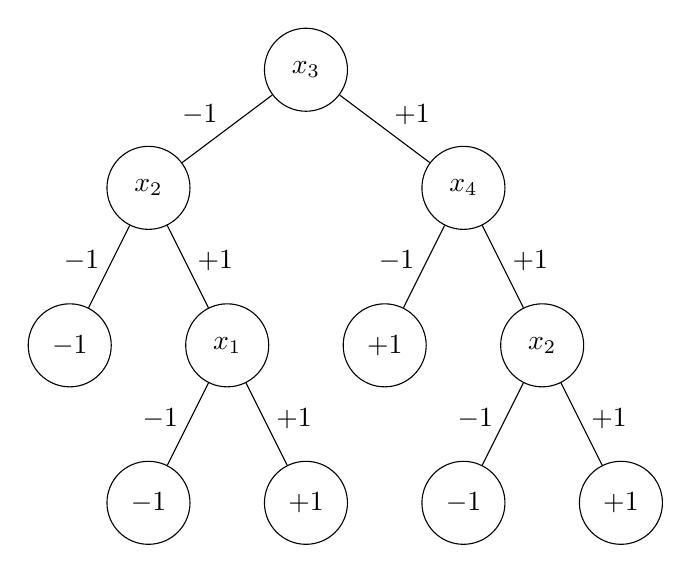
\begin{tikzpicture}
      \node[minimum size=30pt, circle, draw] (root) at (0, 0) {$x_3$};
      \node[minimum size=30pt, circle, draw] (v0) at (-2, -1.5) {$x_2$};
      \node[minimum size=30pt, circle, draw] (v1) at (2, -1.5) {$x_4$};
      \node[minimum size=30pt, circle, draw] (v00) at (-3, -3.5) {$-1$};
      \node[minimum size=30pt, circle, draw] (v01) at (-1, -3.5) {$x_1$};
      \node[minimum size=30pt, circle, draw] (v010) at (-2, -5.5) {$-1$};
      \node[minimum size=30pt, circle, draw] (v011) at (0, -5.5) {$+1$};
      \node[minimum size=30pt, circle, draw] (v10) at (1, -3.5) {$+1$};
      \node[minimum size=30pt, circle, draw] (v11) at (3, -3.5) {$x_2$};
      \node[minimum size=30pt, circle, draw] (v110) at (2, -5.5) {$-1$};
      \node[minimum size=30pt, circle, draw] (v111) at (4, -5.5) {$+1$};
      \draw (root) -- (v0) node[midway, left, yshift=5pt] {$-1$};
      \draw (root) -- (v1) node[midway, right, yshift=5pt] {$+1$};
      \draw (v0) -- (v00) node[midway, left, yshift=2pt] {$-1$};
      \draw (v0) -- (v01) node[midway, right, yshift=2pt] {$+1$};
      \draw (v01) -- (v010) node[midway, left, yshift=2pt] {$-1$};
      \draw (v01) -- (v011) node[midway, right, yshift=2pt] {$+1$};
      \draw (v1) -- (v10) node[midway, left, yshift=2pt] {$-1$};
      \draw (v1) -- (v11) node[midway, right, yshift=2pt] {$+1$};
      \draw (v11) -- (v110) node[midway, left, yshift=2pt] {$-1$};
      \draw (v11) -- (v111) node[midway, right, yshift=2pt] {$+1$};
    \end{tikzpicture}
    \caption{A decision tree.}
    \label{fig:decision-tree}
  \end{figure}
  \item {\bf \em Constant depth circuits.} Recall that a Boolean circuit is a DAG whose vertices are gates which represent operations (e.g., $\wedge, \vee, \neg$), constants ($1, 0$) and variables ($x_1, \ldots, x_n$). We allow each operation to have an unbounded number of inputs; the $\neg$ gate can have only one input. Can we compute the parity (XOR) of $n$ bits in a constant depth with a polynomial-size input for each operation? The answe is ``no,'' which follows from the switching lemma by Furst, Saxe and Sipser.
  
  \begin{theorem}[Hastad, Linial, Mansour and Nisan]
    For any function $f$ computable via a size-$s$ depth-$d$ circuit,
    $$ \sum_{\substack{S \subset [n] \\ |S| > t}} \hat{f}(S)^2 \leq \alpha, $$
    where $t = O(\log (s/\alpha))^{d - 1}$.
  \end{theorem}

  Taking $s = \poly(n)$, $d = O(1)$ and $\alpha = O(\varepsilon)$ implies $t = O(\log^d (n/\varepsilon))$. Therefore, the low degree algorithm gives an $n^{O(\log^d (n/\varepsilon))}$ sample algorithm for learning.
  \item {\bf \em Learning half-spaces.}
  
  \begin{definition}
    For $w \in \RR^n$ and $\theta \in \RR$, the function $h : \{ \pm 1 \}^n \to \{ \pm 1 \}$ defined by $h(x) = \sign(w \cdot x - \theta)$ is called a \emph{half-space function}.
  \end{definition}

  \begin{theorem}
    A half-space function $h : \{ \pm 1 \}^n \to \{ \pm 1 \}$ has Fourier concentration $\alpha(\varepsilon) = c/\varepsilon^2$ for some constant $c$.
  \end{theorem}

  \begin{corollary}
    The low degree algorithm learns half-spaces with $n^{O(1/\varepsilon^2)}$ samples.
  \end{corollary}
\end{enumerate}

\subsection{Noise Sensitivity}

\begin{definition}
  For $\varepsilon \in (0, 1/2)$, the \emph{noise operator} $N_\varepsilon(x)$ randomly flips each bit of $x$ with probability $\varepsilon$, given $x \in \{ \pm 1 \}^n$.
\end{definition}

\begin{definition}
  The \emph{noise sensitivity} of a Boolean function $f : \{ \pm 1 \}^n \to \{ \pm 1 \}$ is defined to be
  $$ \NS_\varepsilon(f) = \PP_{\substack{x \in \{ \pm 1 \}^n \\ \text{noise}}}\left[f(x) \neq f\left(N_\varepsilon(x)\right)\right]. $$
\end{definition}

Following are examples of the noise sensitivity of a Boolean function.

\begin{enumerate}[label=(\roman*)]
  \item If $f(x) = x_1$, then $\NS_\varepsilon(f) = \varepsilon$.
  \item If $f(x) = x_1 \cdots x_k$, then
  \begin{align*}
    \NS_\varepsilon(f) &= \PP[f(x) = \F, f(N_\varepsilon(x) = \T)] + \PP[f(x) = \T, f(N_\varepsilon(x) = \F)] \\
    &= 2\PP[f(x) = \T, f(N_\varepsilon(x) = \F)] \\
    &= 2 \cdot \frac{1}{2^k} \cdot (1 - (1 - \varepsilon)^k).
  \end{align*}
  Therefore, if $\varepsilon \ll 1/k$, then $\NS_\varepsilon(f) \approx \varepsilon k/2^{k - 1}$; if $\varepsilon \gg 1/k$, then $\NS_\varepsilon(f) \approx (1 - e^{-\varepsilon k})/2^{k - 1}$.
  \item If $f(x) = \Maj(x_1, \ldots, x_n)$, then $\NS_\varepsilon(f) = O(\sqrt{\varepsilon})$.
  
  To see this, note that $\Maj(x)$ corresponds to a random walk on a line starting at $0$, and that the location corresponds to the sum of the $x_i$'s so far.

  \begin{fact} \label{fact:random-walk}
    If $X_1, \ldots, X_n \in \{ \pm 1 \}$ are i.i.d\ random variables, then $\EE[|X_1 + \ldots + X_n|] = \sqrt{n}$, and (informally) $|X_1 + \ldots + X_n|$ is likely to be close to $\sqrt{n}$.
  \end{fact}

  Therefore, $N_\varepsilon(x)$ corresponds to a random walk on $\varepsilon n$ bits, where each flip displaces by $\pm 2$. By Fact \ref{fact:random-walk}, the expected displacement is $2\sqrt{\varepsilon n}$.

  Given $x \in \{ \pm 1 \}^n$, we consider the following process:
  \begin{enumerate}[label=\arabic*., itemsep=0pt]
    \item Talk a walk specified by $x$.
    \item Continue the walk according to $2N_\varepsilon(x)$.
  \end{enumerate}

  Pretend that the first walk leaves us at $\sqrt{n}$. By Markov's inequality,
  \begin{align*}
    \PP[\text{the second walk takes us accross $0$}] &= \frac{1}{2} \PP[\text{the second displacement is greater than $\sqrt{n}$}] \\
    &= \frac{1}{2} \cdot \frac{\EE[\text{the second displacement}]}{\sqrt{n}} \\
    &= \frac{1}{2} \cdot \frac{2\sqrt{\varepsilon n}}{\sqrt{n}} = \sqrt{\varepsilon}.
  \end{align*}
  \item {\bf \em Linear threshold functions (half-spaces).}
  
  \begin{theorem}
    If $f$ is a linear threshold function (i.e., a half-space), then $\NS_\varepsilon(f) < 8.8 \sqrt{\varepsilon}$.
  \end{theorem}
  \item {\bf \em Parity functions.}
  
  \begin{proposition}
    Let $S \subset [n]$ be such that $|S| = k$. Then
    $$ \NS_\varepsilon\left(\chi_S\right) = \frac{1 - (1 - 2\varepsilon)^k}{2}. $$
  \end{proposition}

  \item {\bf \em Any function.}
  
  \begin{theorem} \label{thm:noise-sensitivity}
    For any $f : \{ \pm 1 \}^n \to \{ \pm 1 \}$,
    $$ \NS_\varepsilon(f) = \frac{1}{2} - \frac{1}{2} \sum_{S \subset [n]} (1 - 2\varepsilon)^{|S|} \hat{f}(S)^2. $$
  \end{theorem}
  
  The proof of Theorem \ref{thm:noise-sensitivity} is in homework.
\end{enumerate}

Next, we show the relation between noise sensitivity and Fourier concentration.

\begin{theorem} \label{thm:noise-fourier}
  For any $f : \{ \pm 1 \}^n \to \{ \pm 1 \}$ and $\gamma \in (0, 1/2)$,
  $$ \sum_{\substack{S \subset [n] \\ |S| \geq \frac{1}{\gamma}}} \hat{f}(S)^2 < 2.32 \NS_\gamma(f). $$
\end{theorem}

\begin{proof}
  We have
  \begin{align*}
    2\NS_\gamma(f) &= 1 - \sum_{S \subset [n]} (1 - 2\gamma)^{|S|} \hat{f}(S)^2 && \text{(Theorem \ref{thm:noise-sensitivity})} \\
    &= \sum_{S \subset [n]} \left(\hat{f}(S)^2 - (1 - 2\gamma)^{|S|} \hat{f}(S)^2\right) && \text{(Boolean Parseval's identity)} \\
    &= \sum_{S \subset [n]} \left(1 - (1 - 2\gamma)^{|S|}\right) \hat{f}(S)^2 \\
    &\geq \sum_{\substack{S \subset [n] \\ |S| \geq \frac{1}{\gamma}}} \left(1 - (1 - 2\gamma)^\frac{1}{\gamma}\right) \hat{f}(S)^2 \\
    &> \sum_{\substack{S \subset [n] \\ S| \geq \frac{1}{\gamma}}} \left(1 - e^{-2}\right) \hat{f}(S)^2.
  \end{align*}
  Therefore,
  $$ \sum_{\substack{S \subset [n] \\ |S| \geq \frac{1}{\gamma}}} \hat{f}(S)^2 \leq \NS_\gamma(f) \left(\frac{1}{1 - e^{-2}}\right) < 2.32 \NS_\gamma(f). $$
  This completes the proof.
\end{proof}

\begin{corollary}
  For any half-space $h : \{ \pm 1 \}^n \to \{ \pm 1 \}$,
  $$ \sum_{\substack{S \subset [n] \\ |S| \geq O(1/\varepsilon^2)}} \hat{f}(S)^2 \leq \varepsilon. $$
  Therefore, one can learn any half-space from $n^{O(1/\varepsilon^2)}$ random examples.
\end{corollary}

\begin{corollary}
  Any function of $k$ half-spaces can be learned with $n^{O(k^2/\varepsilon^2)}$ samples.
\end{corollary}

\subsection{Learning Heavy Fourier Coefficients}

Given $\theta > 0$ and black box access to $f : \{ \pm 1 \}^n \to \{ \pm 1 \}$, we want to
\begin{enumerate}[label=(\roman*), itemsep=0pt]
  \item output all coefficients $S \subset [n]$ such that $|\hat{f}(S)| \geq \theta$;
  \item only output coefficients $S \subset [n]$ such that $|\hat{f}(S)| \geq \theta/2$.
\end{enumerate}

The main idea is \emph{exhaustive search with good pruning}. The search tree consists of $n$ levels, each representing a variable $x_i$ for $i \in [n]$. For each level $i \in [n]$, going left means $x_i \in S$, and going right means $x_i \not \in S$. Informally, we only go down paths with lots of ``weights,'' and we output leaves reached at the bottom level.

Fix $k \in \{ 0, \ldots, n \}$ representing the current level of search. Fix $S_1 \subset [k]$ representing the current node of search. Let $f_{k, S_1} : \{ \pm 1 \}^{n - k} \to \RR$ be defined by
$$ f_{k, S_1}(x) = \sum_{T \subset \{ k + 1, \ldots, n \}} \hat{f}\left(S_1 \cup T_2\right) \chi_{T_2}(x). $$
Note that we could replace $\chi_{T_2}$ with $\chi_{S_1 \cup T_2} = \chi_{S_1} \cdot \chi_{T_2}$, but $\chi_{S_1}$ remains the same. If $k = 0$, then
$$ f_{0, \emptyset}(x) = \sum_{T_2 \subset [n]} \hat{f}\left(T_2\right) \chi_{T_2}(x) = f(x). $$
On the other hand, if $k = n$, then for any $S_1 \subset [n]$,
$$ f(n, S_1)(x) = \sum_{T_2 \subset \emptyset} \hat{f}\left(S_1 \cup T_2\right) \chi_{T_2}(x) = \hat{f}\left(S_1\right). $$

The plan is to only go down paths with $\EE[f_{k, S_1}(x)^2] \geq \theta^2$. There are several questions to answer:
\begin{enumerate}[label=(\roman*), itemsep=0pt]
  \item Can we compute it?
  \item Does it bring us to right leaves? In other words, do we get to all heavy leaves, and do we get to junks (i.e., light leaves)?
  \item How many paths do we take? In other words, are there a lot of dead ends, and is the running time good?
\end{enumerate}

First, we show that there are not too many paths.

\begin{lemma} \label{lem:not-too-many}
  Let $f : \{ \pm 1 \}^n \to \{ \pm 1 \}$.
  \begin{enumerate}[label=(\roman*), itemsep=0pt]
    \item At most $1/\theta^2$ sets $S \subset [n]$ satisfy $|\hat{f}(S)| \geq \theta$.
    \item For all $k \in \{ 0, \ldots, n \}$, at most $1/\theta^2$ functions $f_{k, S_1}$ have $\EE_{x \in \{ \pm 1 \}^{n - k}}[f_{k, S_1}(x)^2] \geq \theta^2$.
  \end{enumerate}
\end{lemma}

Lemma \ref{lem:not-too-many} implies that our algorithm explores at most $O(1/\theta^2)$ nodes of the search tree.

\begin{proposition} \label{prop:level-parseval}
  For any $k \in \{ 0, \ldots, n \}$ and $S_1 \subset [n]$,
  $$ \EE_{x \in \{ \pm 1 \}^{n - k}} \left[f_{k, S_1}(x)^2\right] = \sum_{T_2 \subset \{ k + 1, \ldots, n \}} \hat{f}\left(S_1 \cup T_2\right)^2. $$
\end{proposition}

\begin{proof}
  we have
  \begin{align*}
    \EE_{x \in \{ \pm 1 \}^{n - k}} \left[f_{k, S_1}(x)^2\right] &= \EE_{x \in \{ \pm 1 \}^{n - k}}\left[\left(\sum_{T_2 \subset \{ k + 1, \ldots, n \}} \hat{f}\left(S_1 \cup T_2\right) \chi_{T_2}\right)^2\right] \\
    &= \EE_{x \in \{ \pm 1 \}^{n - k}}\left[\sum_{T_2, T_2' \subset \{ k + 1, \ldots, n \}} \hat{f}\left(S_1 \cup T_2\right) \hat{f}\left(S_1 \cup T_2'\right) \chi_{T_2}(x) \chi_{T_2'}(x)\right] \\
    &= \sum_{T_2, T_2' \subset \{ k + 1, \ldots, n \}} \hat{f}\left(S_1 \cup T_2\right) \hat{f}\left(S_1 \cup T_2'\right) \EE_{x \in \{ \pm 1 \}^{n - k}}\left[\chi_{T_2}(x) \chi_{T_2'}(x)\right].
  \end{align*}
  Note that
  $$ \EE_{x \in \{ \pm 1 \}^{n - k}}\left[\chi_{T_2}(x) \chi_{T_2'}(x)\right] = \left\{
    \begin{array}{ll}
      0, & \text{if $T_2 \neq T_2'$}, \\
      1, & \text{if $T_2 = T_2'$}.
    \end{array}
  \right. $$
  Therefore,
  $$ \EE_{x \in \{ \pm 1 \}^{n - k}} \left[f_{k, S_1}(x)^2\right] = \sum_{T_2 \subset \{ k + 1, \ldots, n \}} \hat{f}\left(S_1 \cup T_2\right)^2. $$
  This completes the proof.
\end{proof}

\begin{proof}[Proof of Lemma \ref{lem:not-too-many}]
  \begin{enumerate}[label=(\roman*)]
    \item By the Boolean Parseval's identity,
    $$ 1 = \EE_{x \in \{ \pm 1 \}^n}\left[f(x)^2\right] = \sum_{S \subset [n]} \hat{f}(S)^2. $$
    Therefore, if more than $1/\theta^2$ sets $S \subset [n]$ had $|\hat{f}(S)| \geq \theta$, then
    $$ \sum_{S \subset [n]} \hat{f}(S)^2 > \frac{1}{\theta} \cdot \theta^2 = 1, $$
    a contradiction.
    \item Let $k \in \{ 0, \ldots, n \}$. 

    Therefore,
    \begin{align*}
      1 &= \sum_{S \subset [n]} \hat{f}(S)^2 && \text{(Boolean Parseval's identity)} \\
      &= \sum_{S_1 \subset [k]} \sum_{T_2 \subset \{ k + 1, \ldots, n \}} \hat{f}\left(S_1 \cup T_2\right)^2 \\
      &= \sum_{S_1 \subset [k]} \EE_{x \in \{ \pm 1 \}^{n - k}}\left[f_{k, S_1}(x)^2\right] && \text{(Proposition \ref{prop:level-parseval})}
    \end{align*}
    Therefore, at most $1/\theta^2$ sets $S_1 \subset [k]$ have $\EE_{x \pm \{ \pm 1 \}^{n - k}}[f_{k, S_1}(x)^2] \geq \theta^2$.
  \end{enumerate}
\end{proof}

Second, we show that the algorithm does not miss out heavy Fourier coefficients. To see this, for any $k \in \{ 0, \ldots, n \}$ and $S_1 \subset [k]$, if there exists $T_2^* \subset \{ k + 1, \ldots, n \}$ such that $|\hat{f}(S_1 \cup T_2^*)| > \theta$, then Proposition \ref{prop:level-parseval} implies that
$$ \EE_{x \in \{ \pm 1 \}^n}\left[f_{k, S_1}(x)^2\right] = \sum_{T_2 \subset \{ k + 1, \ldots, n \}} \hat{f}\left(S_1 \cup T_2\right)^2 \geq \hat{f}\left(S_! \cup T_2^*\right) \geq \theta^2. $$
To avoid outputting junks (i.e., light Fourier coefficients), we add a simple fix to the algorithm: For each candidate to $S$, estimate its Fourier coefficient and make sure it is big enough before outputting it.

\begin{lemma} \label{lem:estimate}
  For $x \in \{ \pm 1 \}^{n - k}$,
  $$ f_{k, S_1}(x) = \EE_{y \in \{ \pm 1 \}^k}\left[f(yx) \chi_{S_1}(y)\right], $$
  where $yx$ denotes the concatenation operation.
\end{lemma}

By Lemma \ref{lem:estimate}, we can estimate $f_{k, S_1}(x)$ by picking random $y$, outputting the average and using the Chernoff bound.

\begin{proof}
  Let $x \in \{ \pm 1 \}^{n - k}$. Then
  $$ f(yx) = \sum_{T \subset [n]} \hat{f}(T) \chi_T(yx). $$
  Since $T = T_1 \cup T_2$ where $T_1 \subset [k]$ and $T_2 \subset \{ k + 1, \ldots, n\}$, then $\chi_T(yx) = \chi_{T_1}(y) \chi_{T_2}(x)$. Therefore,
  \begin{align*}
    \EE_{y \in \{ \pm 1 \}^k}\left[f(yx) \chi_{S_1}(y)\right] &= \EE_{y \in \{ \pm 1 \}^k}\left[\sum_{T_1 \subset [k]} \sum_{T_2 \subset \{ k + 1, \ldots, n \}} \hat{f}\left(T_1 \cup T_2\right) \chi_{T_1}(y) \chi_{T_2}(x) \chi_{S_1}(y)\right] \\
    &= \sum_{T_1 \subset [k]} \sum_{T_2 \subset \{ k + 1, \ldots, n \}} \hat{f}\left(T_1 \cup T_2\right) \chi_{T_2}(x) \EE_{y \in \{ \pm 1 \}^k}\left[\chi_{T_1}(y) \chi_{S_1}(y)\right].
  \end{align*}
  Note that
  $$ \EE_{y \in \{ \pm 1 \}^k}\left[\chi_{T_1}(y) \chi_{S_1}(y)\right] = \left\{
    \begin{array}{ll}
      0, & \text{if $T_1 \neq S_1$}, \\
      1, & \text{if $T_1 = S_1$}.
    \end{array}
  \right. $$
  Therefore,
  $$ \EE_{y \in \{ \pm 1 \}^k}\left[f(yx) \chi_{S_1}(y)\right] = \sum_{T_2 \subset \{ k + 1, \ldots, n \}} \hat{f}\left(S_1 \cup T_2\right) \chi_{T_2}(x) = f_{k, S_1}(x). $$
  This completes the proof.
\end{proof}

Now we are ready to summarize the full algorithm, called the Kushilevitz-Mansour algorithm, in Algorithm \ref{alg:km}.

\begin{algorithm}
  \If(\CommentSty{(leaf)}){$k = n$}{
    \If{the $\theta/4$-additive estimate of $\hat{f}(S_1)$ is at least $3/4$}{
      \Return{$S_1$}
    }
  }
  \ElseIf(\CommentSty{(check left subtree)}){$\EE_{x \in \{ \pm 1 \}^{n - k}}[f_{k, S_1 \cup \{ k + 1 \}}(x)^2] \geq \theta^2/2$}{
    recurse on $(k + 1, S_1 \cup \{ k + 1 \})$
  }
  \ElseIf(\CommentSty{(check right subtree)}){$\EE_{x \in \{ \pm 1 \}^{n - k}}[f_{k, S_1}(x)^2] \geq \theta^2/2$}{
    recurse on $(k + 1, S_1)$
  }
  \caption{The Kushilevitz-Mansour algorithm, given the current level $k \in \{ 0, \ldots, n \}$ and the current prefix $S_1 \subset [n]$.}
  \label{alg:km}
\end{algorithm}

The Kushilevitz-Mansour algorithm has the following applications:
\begin{enumerate}[label=(\roman*), itemsep=0pt]
  \item Learn decision trees of size $\leq t$ (not just small depth);
  \item functions of small $L_1$-norm, where the \emph{$L_1$-norm} of a function $f : \{ \pm 1 \}^n \to \{ \pm 1 \}$ is defined to be $L_1(f) = \sum_{S \subset [n]} |\hat{f}(S)|$ (by setting $\theta \leftarrow \varepsilon/L_1(f)$).
\end{enumerate}

\section{Monotone Functions}

\begin{definition}
  We define $\preccurlyeq$ to be a partial order over $\{ \pm 1 \}^n$ such that $x \leq y$ if and only if $x_i \leq y_i$ for all $i \in [n]$.
\end{definition}

\begin{definition}
  A Boolean function $f : \{ \pm 1 \}^n \to \{ \pm 1 \}$ is \emph{monotone} if $f(x) \leq f(y)$ for all $x, y \in \{ \pm 1 \}^n$ with $x \preccurlyeq y$.
\end{definition}

Are monotone functions learnable? Occam's Razor implies that $O(\log|\mathcal C|)$ samples suffice, where $\mathcal C$ is the class of monotone functions. We have the following lower bound on $|\mathcal C|$: Consider \emph{slice functions} which have values $+ 1$ on level greater than $n/2$ in the Boolean hypercube, values $-1$ on level less than $n/2$, and arbitrary values on level $n/2$. Then slice functions are all monotone. There are $\binom{n}{n/2}$ nodes on level $n/2$, so there are $2^{\binom{n}{n/2}}$ monotone functions. Therefore, the sample complexity implied by Occam's Razor is $O(\binom{n}{n/2}) = O(2^n/\sqrt{n})$. In homework, we shall show that $2^{O(\sqrt{n})}$ samples suffice.

We show that monotone functions have weak agreement with some dictator function.

\begin{theorem} \label{thm:monotone-dictator}
  For any monotone Boolean function $f : \{ \pm 1 \}^n \to \{ \pm 1 \}$, there exists $g \in S := \{ \pm 1, x_1, x_2, \ldots, x_n \}$ such that
  $$ \PP_{x \in \{ \pm 1 \}^n}[f(x) = g(x)] \geq \frac{1}{2} + \Omega\left(\frac{1}{n}\right). $$
\end{theorem}

Note that if we add the majority function to $S$, then we can get $1/2 + O(1/\sqrt{n})$. Theorem \ref{thm:monotone-dictator} suggests the following learning algorithm: Estimate the agreement of $f$ with each member of $S$, and output the best.

If $f$ has weak agreement with $+1$ or $-1$, then we are done. Otherwise, $\PP[f(x) = 1] \in [1/4, 3/4]$. Consider a ``graphic'' view of the Boolean hypercube in Figure \ref{fig:monotone-hypercube}, where vertices with value $1$ are colored red and vertices with value $-1$ are colored blue.

\begin{figure}[h]
  \centering
  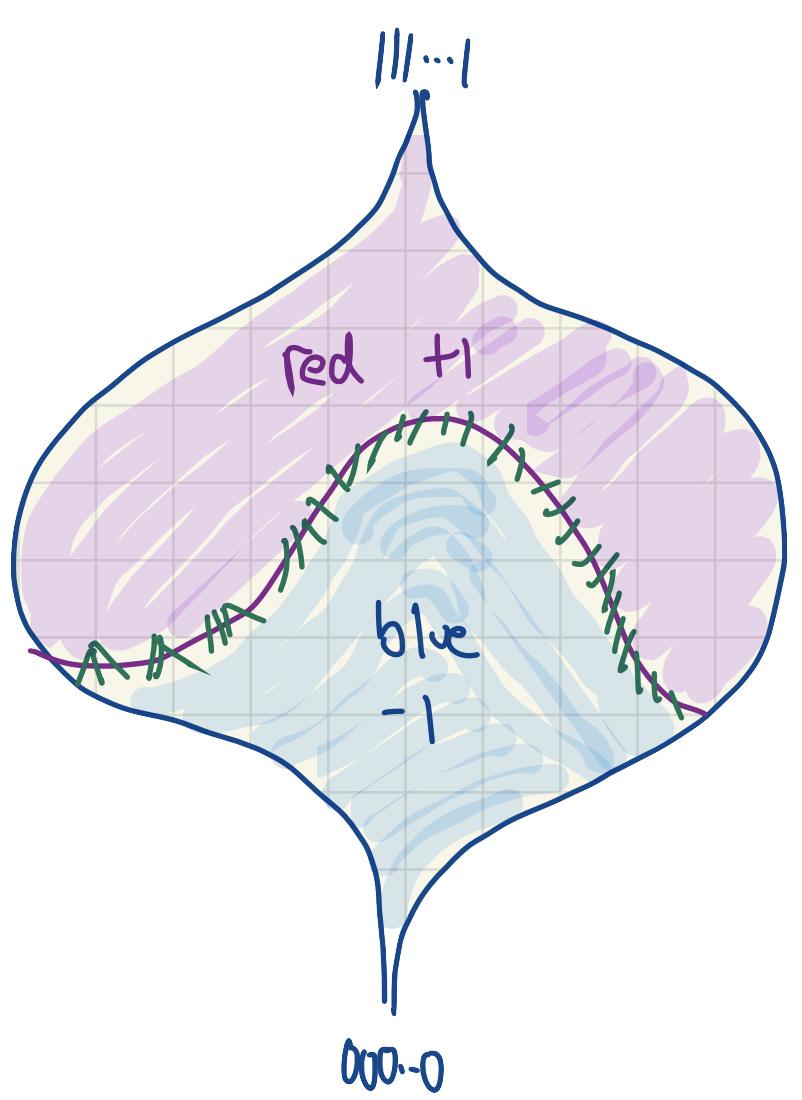
\includegraphics[width=.4\textwidth]{figures/hypercube.png}
  \caption{A ``graphic'' view of the Boolean hypercube, where vertices with value $1$ are colored red and vertices with value $-1$ are colored blue.}
  \label{fig:monotone-hypercube}
\end{figure}

\begin{definition}
  Let $f : \{ \pm 1 \}^n \to \{ \pm 1 \}$ be a monotone Boolean function. The \emph{influence of $f$ at the $i^\text{th}$ direction} is defined to be
  $$ \Inf_i(f) = \frac{\text{\# red-blue edges in the $i^\text{th}$ direction}}{2^{n - 1}} = \PP_{x \in \{ \pm 1 \}^n}\left[f(x) \neq f\left(x^{\oplus i}\right)\right], $$
  where $x^{\oplus i}$ is the vector obtained by flipping the $i^\text{th}$ bit in $x$. The \emph{influence} of $f$ is defined to be
  $$ \Inf(f) = \frac{\text{\# red-blue edges}}{2^n} = \sum_{i = 1}^n \Inf_i(f). $$
\end{definition}

\begin{theorem} \label{thm:inf-i}
  Any monotone Boolean function has $\Inf_i(f) = \hat{f}(\{ i \})$.
\end{theorem}

\begin{theorem} \label{thm:majority}
  The majority function $f(x) := \sign(\sum_{i = 1}^n x_i)$, where $n$ is odd, maximizes the influence among monotone functions.
\end{theorem}

Theorems \ref{thm:inf-i} and \ref{thm:majority} will be proved in homework. By Theorem \ref{thm:inf-i}, any monotone Boolean function $f$ has
$$ \Inf_i(f) = \hat{f}(\{ i \}) = 2\PP_{x \in \{ \pm 1 \}^n}\left[f(x) = \chi_{\{ i \}}(x)\right] - 1 = 2\PP_{x \in \{ \pm 1 \}^n}\left[f(x) = x_i\right] - 1. $$
Therefore, showing $\Inf_i(f) \geq \Omega(1/n)$ is equivalent to showing
$$ \PP_{x \in \{ \pm 1 \}^n} \geq \frac{1}{2} + \frac{\Inf_i(f)}{2} = \frac{1}{2} + \Omega\left(\frac{1}{n}\right). $$
Hence, such an index $i \in [n]$ would prove Theorem \ref{thm:monotone-dictator}.

We introduce the \emph{canonical path argument}, which proceeds as follows:
\begin{enumerate}[label=(\roman*), itemsep=0pt]
  \item Define the canonical path for every red-blue pair of vertices (which must cross at least one red-blue edge).
  \item Show an upper bound on the number of canonical paths passing through any edge (called \emph{bounding the congestion}).
  \item Conclude a lower bound on the number of red-blue edges.
\end{enumerate}

First, we define the canonical path for every red-blue pair of vertices.

\begin{definition}
  For all $(x, y) \in \{ 0, 1 \}^n \times \{ 0, 1 \}^n$ such that $x$ is red and $y$ is blue, the \emph{canonical path} from $x$ to $y$ is defined by the following procedure: Scan bits from left to right, and flip where needed. Each flip corresponds to a step in the canonical path (in the undirected Boolean hypercube).
\end{definition}

Note that if $x$ is red and $y$ is blue, then the canonical path from $x$ to $y$ must include some red-blue edge. Recall that $\PP[f(x) = 1] \in [1/4, 3/4]$, then the number of red-blue $(x, y)$ pairs that have canonical paths is at least
$$ \left(\frac{1}{4} \cdot 2^n\right) \cdot \left(\frac{1}{4} \cdot 2^n\right) = \frac{1}{16} \cdot 2^{2n}. $$

Second, we show an upper bound on the number of canonical paths passing through any (red-blue) edge. Note that any red-blue pair $(x, y)$ taking edge $(u, u^{\oplus i})$ must have
\begin{align*}
  y_1 \ldots y_{i - 1} y_i &= u_1 \ldots u_{i - 1} \overline{u_i}, \\
  x_i x_{i + 1} \ldots x_n &= u_i u_{i + 1} \ldots u_n.
\end{align*}
Hence, we can pick $y_{i + 1}, \ldots, y_n$ and $x_1, \ldots, x_{i - 1}$ freely, so there are at most $2^n$ total choices.

Third, since each red-blue canonical path crosses at least one red-blue edge,
$$ (\text{\# red-blue edges}) \cdot (\text{max \# canonical paths using each edge}) \geq \text{\# red-blue canonical paths}. $$
Therefore, the number of red-blue edges is at least
$$ \frac{\frac{1}{16} \cdot 2^{2n}}{2^n} = \frac{1}{16} \cdot 2^n. $$
It follows that there exists $i \in [n]$ such that there exist at least $2^n/(16n)$ red-blue edges in the $i^\text{th}$ direction, so
$$ 2\PP_{x \in \{ \pm 1 \}^n}\left[f(x) = x_i\right] - 1 = \hat{f}(\{ i \}) = \Inf_i(f) \geq \frac{\frac{2^n}{16n}}{2^{n - 1}} = \frac{1}{8n}. $$
This proves that there exists $i \in [n]$ such that $\PP_{x \in \{ \pm 1 \}^n}[f(x) = x_i] \geq 1/2 + 1/(16n)$.

\section{Weak and Strong Learning}

\begin{definition}
  An algorithm $\mathcal A$ \emph{weakly PAC learns} a concept class $\mathcal C$ if there exists $\gamma > 0$ such that for any $C \in \mathcal C$, distribution $\mathcal D$ and $\delta > 0$, with probability at least $1 - \delta$, given $\Ex_\mathcal{D}(C)$, $\mathcal A$ outputs $h$ such that
  \begin{equation} \label{eq:weak}
    \error_{\mathcal D}(h) := \PP_{x \sim \mathcal D}[h(x) \neq C(x)] \leq \frac{1}{2} - \frac{\gamma}{2}.
  \end{equation}
  Here, $\gamma/2$ is called the \emph{advantage over guessing}.
\end{definition}

Note that we used to ask for $\PP_{x \sim \mathcal D}[h(x) = C(x)] \geq 1 - \varepsilon$ for all $\varepsilon > 0$; this is called \emph{(strong) PAC learning}.

\begin{theorem} \label{thm:weak-strong}
  If a concept class $\mathcal C$ can be weakly learned on any distribution $\mathcal D$, then $\mathcal C$ can be (strongly) learned, i.e., with error at most $\varepsilon$ for all $\varepsilon > 0$.
\end{theorem}

We are interested in the dependence of the running time of learning on $\gamma$, $\delta$ and $\varepsilon$. The plan for the proof of Theorem \ref{thm:weak-strong} is as follows:
\begin{enumerate}[label=(\roman*), itemsep=0pt]
  \item \label{item:modest} ``Modest'' accuracy boosting.
  \item Recursively use \ref{item:modest} to drive down error.
\end{enumerate}

First, we present a modest accuracy boosting algorithm in Algorithm \ref{alg:modest}, given an example oracle $\Ex_{\mathcal D}(f)$ to $f$ with distribution $\mathcal D$ and a weak learner $\WL$. Let
\begin{align*}
  \beta_1 &= \PP_{x \in \mathcal D}\left[h_1(x) \neq f(x)\right], \\
  \beta_2 &= \PP_{x \in \mathcal D_2}\left[h_2(x) \neq f(x)\right], \\
  \beta_3 &= \PP_{x \in \mathcal D_3}\left[h_3(x) \neq f(x)\right],
\end{align*}
We observe that if $h_1(x) = f(x)$, then $\mathcal D(x) = 2(1 - \beta_1) \mathcal D_2(x)$ (i.e., $\mathcal D_2(x) = \mathcal D(x) \cdot 1/(2(1 - \beta_1))$); if $h_1(x) \neq f(x)$, then $\mathcal D(x) = 2\beta_1 \mathcal D_2(x)$. See Figure \ref{fig:modest} for an illustration. Moreover, we divide $\mathcal D_2$ into four regions in Table \ref{tab:regions}, also illustrated in Figure \ref{fig:modest}. We have the following lemma, the proof of which we omit for now.

\begin{lemma}
  $\error_{\mathcal D}(h) \leq g(\beta) := 3\beta^3 - 2\beta^3$.
\end{lemma}

\begin{algorithm}[h]
  $h_1 \leftarrow \text{run $\WL$ on $\mathcal D$ for function $f$}$ \\
  create a distribution $\mathcal D_2$ by flipping a coin such that \\
  {\Indp\If{head}{
    draw examples from $\mathcal D$ until finding $x$ such that $h_1(x) = f(x)$ \CommentSty{($h_1$ is correct)} \\
    output $x$
  }
  \Else{
    draw examples from $\mathcal D$ until finding $x$ such that $h_1(x) \neq f(x)$ \CommentSty{($h_1$ is incorrect)} \\
    output $x$
  }}
  $h_2 \leftarrow \text{run $\WL$ on $\mathcal D_2$ for function $f$}$ \CommentSty{($\error_{\mathcal D_2}(h_1) = 1/2$)} \\
  create a distribution $\mathcal D_3$ by drawing examples from $\mathcal D$ until finding $x$ with $h_1(x) \neq h_2(x)$ \\
  $h_3 \leftarrow \text{run $\WL$ on $\mathcal D_3$ for function $f$}$
  \caption{A modest accuracy boosting algorithm, given an example oracle $\Ex_{\mathcal D}(f)$ to $f$ with distribution $\mathcal D$ and a weak learner $\WL$.}
  \Return{$\Maj(h_1, h_2, h_3)$} \CommentSty{(on $x$, compute $h_1(x), h_2(x), h_3(x)$, output majority answer)}
  \label{alg:modest}
\end{algorithm}

\begin{figure}[h]
  \centering
  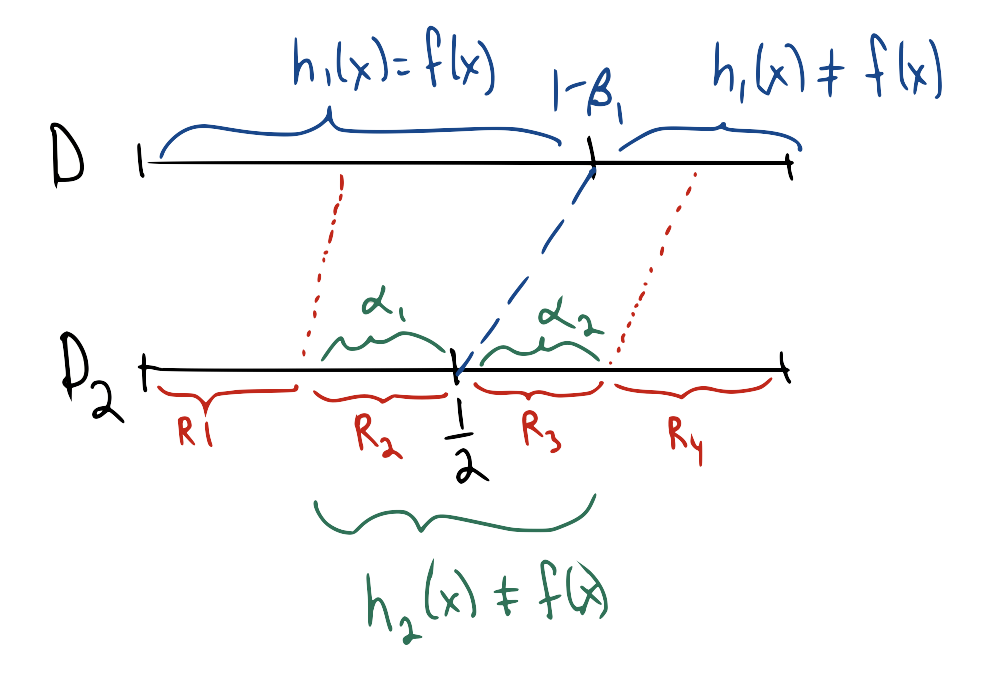
\includegraphics[width=.5\textwidth]{figures/modest.png}
  \caption{Illustrating the analysis of Algorithm \ref{alg:modest}.}
  \label{fig:modest}
\end{figure}

\begin{table}[h]
  \centering
  \begin{tabular}{l|l|l}
    $R_1$ & $h_1(x) = h_2(x) = f(x)$ & $\Maj(h_1, h_2, h_3)$ is correct \\
    \hline
    $R_2$ & $h_1(x) = f(x) \neq h_2(x)$ & maybe $h_3$ helps? \\
    \hline
    $R_3$ & $h_1(x) = h_2(x) \neq f(x)$ & $\Maj(h_1, h_2, h_3)$ is incorrect \\
    \hline
    $R_4$ & $h_1(x) \neq h_2(x) = f(x)$ & maybe $h_3$ helps?
  \end{tabular}
  \caption{Four regions of $\mathcal D_2$.}
  \label{tab:regions}
\end{table}

Second, we give a recursive accuracy boosting algorithm in Algorithm \ref{alg:recursive}. We illustrate the recursion from Algorithm \ref{alg:recursive} in Figure \ref{fig:recursion}.

\begin{algorithm}[h]
  \If{$\rho$ is already good enough}{
    \Return{$\WL$ on $\mathcal D'$}
  }
  $\beta \leftarrow g^{-1}(\rho)$ \CommentSty{(error bound requried from below to get error $\rho$)} \\
  define $\mathcal D_2'$ and $\mathcal D_3'$ as in Algorithm \ref{alg:modest} \\
  \ForEach{$i \in [3]$}{
    $h_i \leftarrow \SL(\beta, \mathcal D_i')$
  }
  \Return{$\Maj(h_1, h_2, h_3)$}
  \caption{A recursive accuracy boosting algorithm $\SL$, given required error $\rho$ and distribution $\mathcal D'$.}
  \label{alg:recursive}
\end{algorithm}

\begin{figure}[h]
  \centering
  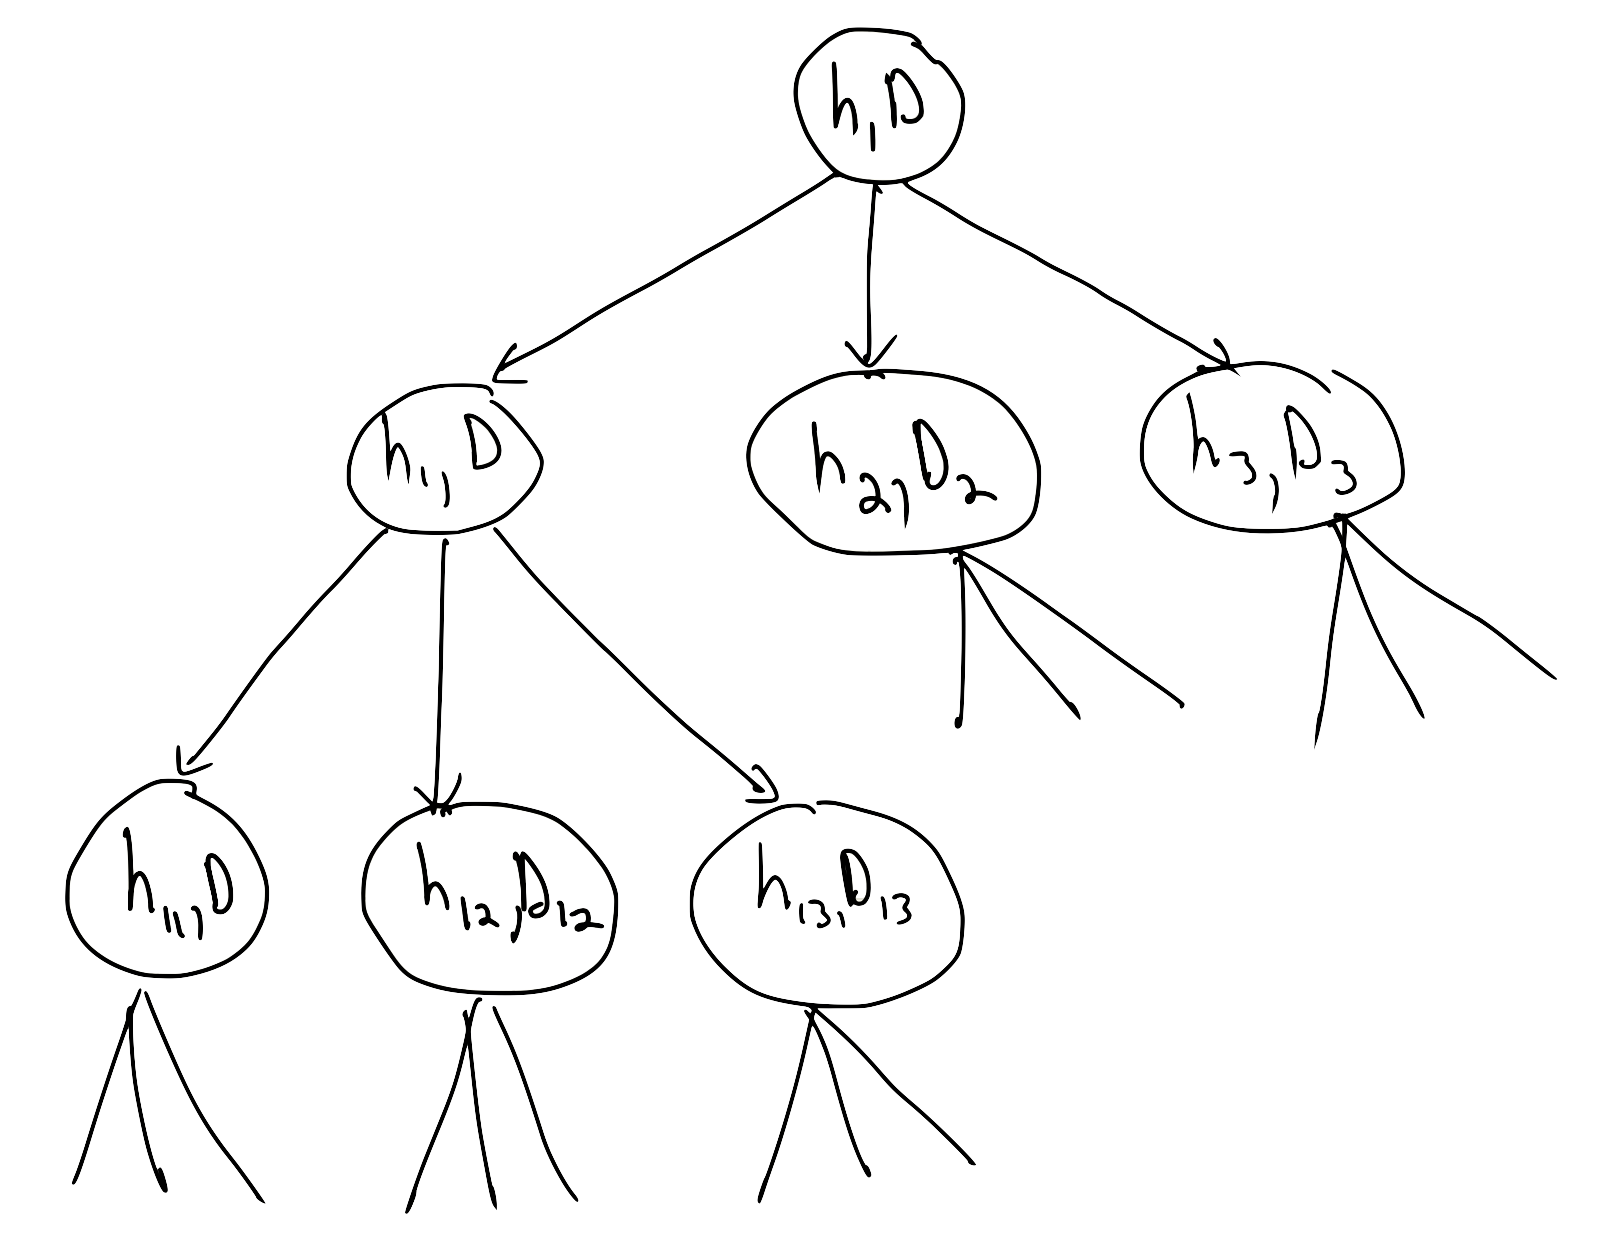
\includegraphics[width=0.6\textwidth]{figures/recursion.png}
  \caption{Illustrating the recursion of Algorithm \ref{alg:recursive}.}
  \label{fig:recursion}
\end{figure}

\begin{corollary}
  If a concept class $\mathcal C$ is learnable, then any concept $C \in \mathcal C$ has a polynomial size circuit.
\end{corollary}

\begin{theorem}
  Suppose that a function $f$ cannot be computed by polynomial size circuits. Then there exists a distribution $\mathcal D$ such that $f$ is \emph{average-case hard} on $\mathcal D$ (i.e., there exists no polynomial size circuit that gets it right more than $1/2$ in time $1/\poly(n)$).
\end{theorem}

\end{document}
